\documentclass[10pt,a4paper,twocolumn]{article}
\usepackage[margin=18mm,columnsep=7mm]{geometry}
\usepackage[T1]{fontenc}
\usepackage[utf8]{inputenc}
\usepackage{lmodern,microtype}
\usepackage{amsmath,amssymb,amsthm,bm}
\usepackage{graphicx,booktabs,array,tabularx,multirow}
\usepackage[font=small,labelfont=bf]{caption}
\usepackage{enumitem}
\usepackage{xurl}
\usepackage[colorlinks=true,allcolors=blue]{hyperref}
\usepackage{balance}
\usepackage{placeins}
\renewcommand{\topfraction}{0.95}
\renewcommand{\dbltopfraction}{0.95}
\renewcommand{\textfraction}{0.05}
\renewcommand{\floatpagefraction}{0.75}
\renewcommand{\dblfloatpagefraction}{0.75}
\setcounter{topnumber}{3}
\setcounter{dbltopnumber}{3}
\setlength{\parskip}{2pt}
\setlength{\emergencystretch}{1.5em}
\setlist[itemize]{leftmargin=*,nosep}
\newcommand{\E}{\mathbb E}
\newcommand{\Prb}{\mathbb P}
\newcommand{\R}{\mathbb R}
\newcommand{\1}{\mathbf 1}
% Primitive input keeps file-hook tokens outside tabular row alignment.
\newcommand{\inputtablerows}[1]{\csname @@input\endcsname #1 }
\newtheorem{proposition}{Proposition}
\title{\vspace{-7mm}Deadline-aware formation adaptation for surface-vehicle monitoring:\\
economic control and tests of biological proposal mechanisms}
\author{5.9.1. MARIN\\[-1mm]\small USV swarm project}
\date{\small Research manuscript, version 4, 7 September 2026}
\hypersetup{pdfauthor={5.9.1. MARIN},pdftitle={Deadline-aware formation adaptation for surface-vehicle monitoring},pdfsubject={Synthetic maritime monitoring research; version 4}}
\begin{document}
\maketitle
\begin{abstract}
Surface-vehicle monitoring requires sensed reports to arrive on time while formation changes consume time and energy. We develop a local economic controller with correlated sensing and radio outages, temporal multihop delivery, delayed observations and finite movement. In 960 held-out one-hour missions, it improves delivered coverage by 0.95 percentage points relative to a separately selected static ring; relative to an earlier formation-library controller, coverage increases by 1.69 points and mean energy decreases by 62.5\%. Small fungal-transport gains fail robustness checks. A further 576-mission main study tests reciprocal movement timing and nonlinear proposal inhibition against matched controls. Reciprocal minus periodic handover changes coverage by -0.21 [-0.35, -0.09] points; nonlinear minus linear inhibition changes it by +0.01 [-0.04, +0.06] points. Additional model-shift and integration diagnostics retain negative comparisons. Three 2048-step PPO pilots change mean interval reward by -0.00607 [-0.00743, -0.00449] relative to a development-selected constant setting on unseen missions. Intervals are paired 95\% bootstrap intervals conditional on the evaluated controllers. The contribution is an inspectable testbed and controlled mechanism comparisons, not a first-use claim, a field-validated system or a demonstrated general advantage of biological or learned control.

\end{abstract}
\noindent\textbf{Keywords:} unmanned surface vessels; delivered sensing coverage;
temporal networks; age of information; biological transport networks;
formation adaptation; reproducible simulation.

\section{Introduction}
An unmanned surface vessel (USV) can detect an event without delivering a useful
report to its coordinator. Waves can reduce visibility, radio conditions can
interrupt a relay path, and a command can arrive after the geometry that motivated
it has changed. Expanding a formation may improve sensing while weakening delivery;
contracting it may restore radio links while leaving monitoring gaps. The relevant
control question is therefore not simply whether the vessels cover an area or
whether a graph is connected. It is whether changing their physical positions
improves timely information at an acceptable movement cost.

Coverage control has a substantial established literature, including distributed
locational optimization~\cite{cortes2004} and heterogeneous sensing
capabilities~\cite{santos2018}. Biological motivation is also established in USV
control: constrained waterjet-USV formation control using bioinspired
neurodynamics predates this work~\cite{wang2019}. A recent UAV study jointly treats
information age, reliability and connectivity~\cite{bafarassat2026}. Accordingly,
neither adaptive coverage, biological inspiration, nor their broad combination
with connectivity is claimed here as a new research area.

This study addresses a narrower engineering question. When sensing and
communication share environmental disturbances, can a controller use
deadline-respecting delivery estimates to decide \emph{which small formation
changes are worth executing}? We also ask whether two recent biological ideas
offer useful movement proposals: branching/fusion in fungal transport networks,
and interaction-dependent movement heterogeneity in foraging ants. A second, separately frozen study tests reciprocal movement timing and nonlinear option inhibition, and evaluates three short PPO training runs against all nine constant high-level settings.

The contribution is an inspectable synthesis and its controlled evaluation:
(i) a common economic acceptance rule with finite movement forecasts;
(ii) an explicit transfer from hydraulic link importance to deadline-dependent
radio-link importance; and (iii) paired tests against a development-selected
static formation and conventional local controls. The Bernoulli sensitivity
identity and resistor-network differentiation used in the transfer are standard
mathematical tools, not newly discovered theorems. Whether the resulting
combination merits a publishable novelty claim depends on comparison with further
close prior art and validation beyond the synthetic setting.

\section{Related work and biological transfer}
\subsection{Coverage, communications and dynamics}
Classical coverage methods connect vehicle positions to spatial sensing costs;
heterogeneous formulations allow different sensing modalities or capabilities
to receive different spatial responsibilities~\cite{cortes2004,santos2018}.
Those ideas motivate a conventional coverage-gradient comparator, but a spatial
coverage score alone does not describe a report's arrival before a deadline.

The age-of-information (AoI) framework measures the elapsed time since the source
timestamp of the newest update received at a monitor~\cite{yates2016}. The present
primary outcome is a weighted deadline-violation complement, rather than mean AoI.
It is sensitive to both sensing failures and time-ordered relay opportunities.
Bafarassat and Coleri's 2026 preprint couples UAV information urgency and
connectivity using successive convex approximation and finite-blocklength
reliability~\cite{bafarassat2026}. Its stated architecture forwards sensed payloads
directly to a fusion center while inter-UAV links support coordination. The present
simulator explicitly caches and forwards reports over changing multihop paths.
This distinction identifies a modeling focus; it does not establish superiority
over that method. We do not reproduce its optimization problem or claim a
state-of-the-art benchmark against it.

For physical deployment, surface-craft dynamics are naturally represented by
inertia, Coriolis, damping and forcing terms in a marine-craft
model~\cite{fossen2021}. Our simulator instead uses a simpler planar guidance and
response model. Its controlled stochastic comparisons are useful for evaluating
high-level decisions, but its energy and weather curves must be fitted before
they can support vessel-specific operational claims.

\subsection{Fungal construction and transport}
Oyarte Galvez et al.\ observed expanding fungal networks with a pulse of growing
tips followed by a saturating filament-density wave~\cite{oyarte2025}. Their
branching and annihilating range-expansion model couples tip density $n$ and
filament density $\rho$:
\begin{align}
 \partial_t n &= b(n)-a(n,\rho)+\nabla\cdot \bm J(n),\\
 \partial_t \rho &= vn .
\end{align}
Linear branching $b(n)=\alpha n$ and density-dependent anastomosis
$a(n,\rho)=\beta n\rho$ are compatible with the observed wave behavior.
A 2026 preprint by Lucas et al.\ studies local branching, fusion and stopping
rules under a fixed network-length budget, comparing the generated networks
with biological multi-objective trade-offs~\cite{lucas2026}. Related physical
work explains loop formation near network breakthrough~\cite{zukowski2024}.

These observations suggest separating sensing expansion from transport repair.
However, a fixed-size USV team cannot reproduce by branching, leave permanent
conducting filaments behind, or fuse its hulls. We therefore transfer
\emph{proposal roles}: a branching direction increases prospective sensing;
a fusion direction improves transport; a stopping rule rejects an unprofitable
reconfiguration. No fungal growth equation is asserted to govern vessel motion.
No biological Pareto-optimality result is inherited by the controller.

Adjacent biological transport-network inspiration is already robot-networking
prior art. Martinelli
et al.\ describe a Physarum-inspired mesh mechanism in a simulated port with
three mobile robots~\cite{martinelli2026}. This comparison concerns a transport
analogy; Physarum is a slime mould, whereas the branching/fusion growth studies
above concern fungi. We do not claim first use of biological transport
inspiration in robot communication. The specific question here is
whether link reinforcement should be driven by expected timely report delivery,
including the physical cost of changing the radio geometry.

\subsection{Ant movement heterogeneity}
Fernandez-Lopez et al.\ study how heterogeneous movement and information transfer
shape foraging efficiency in \emph{Aphaenogaster senilis}, interpreted through a
liquid-brain framework~\cite{fernandez2025}. We use this as motivation for
recruiting a subset of vessels into a new excursion. The implemented activity,
refractory and coupling equations are stated below and are our engineering
adaptation. They are not a reproduction of the authors' ant simulator.
In particular, nominal radio weights are not physical antennal contacts.

The literature search used primary research, author-hosted papers and official
documentation, with focused searches through 7 September 2026. The accessible
ant paper metadata/abstract and author explanation support the qualitative
motivation; its full mathematical supplement could not be retrieved. A claim
that no robot or drone study has tried an equivalent rule would be unjustified.
The release includes a source ledger explaining these boundaries.

\section{Problem and simulation model}
\subsection{A receiver-side mission objective}
Let $p_i(t)\in\R^2$ be the position of vessel $i=1,\ldots,N$, with a base at
the origin. Monitoring points $x_m$ sample three concentric annuli at
$0.9R,R,1.1R$, with normalized priority weights $w_m(t)$. This is quadrature of
an \emph{annular monitoring distribution}; it is not an estimate of Cartesian
area coverage over an entire disk.

Let $\tau_m^b(t)$ be the source timestamp of the newest report for point $m$
available at the base. Define
\begin{align}
 A_m(t)&=t-\tau_m^b(t),\\
 C(t)&=\sum_m w_m(t)\1\{A_m(t)\leq D\},\label{eq:C}\\
 \bar C&=\frac{1}{T-t_w}\int_{t_w}^{T}C(t)\,dt .
\end{align}
Never-received reports have infinite age. Actual implementation averages the
discrete samples with $t\geq t_w$, including the endpoint at warm-up. We also
report AoI clipped at $10D=300$ s, its saturation fraction, and fleet energy
$E=\sum_i\int_0^T P_i(t)\,dt/3600$ in Wh. Deployment energy is included.
The primary metric concerns delivered freshness, not guaranteed target tracking,
classification correctness, or collision safety.

\subsection{Sensing and environmental dependence}
A synthetic severity $s(t)\in[0,1]$ changes nominal sensing ranges and visibility.
It is not a calibrated sea-state number. The nominal radar half-range is
$r_r(s)=1650\exp(-1.4s)$ m and the camera half-range is
$r_c(s)=650\exp(-0.8s)$ m. Radar range additionally depends on bearing relative
to wind and an unknown vessel-specific multiplier $\theta_i$.
For logistic roll-off $\sigma$, radar conditional detection is
\begin{equation}
 p^r_{im}=0.94\,\sigma\!\left(\frac{r_{im}-d_{im}}{0.2r_{im}}\right),
\end{equation}
with an analogous camera curve of peak 0.86 and relative width 0.22.
Conditional sensor fusion is $p_{im}=1-(1-p^r_{im})(1-p^c_{im})$.
A single visibility variable $V_i(t)$ gates \emph{both} sensors on a vessel;
their obscuration failures are not treated as independent.

Visibility follows a correlated Gaussian field with a shared spatial component
and vessel-specific response, transformed to a Bernoulli variable with
availability
\begin{equation}
 a_i(s)=\sigma\!\left(\operatorname{logit}
 \frac{0.94}{1+1.1s^2}+b_i\right).
\end{equation}
The simulator uses a random Fourier spatial field and a 15 s default temporal
memory. The planner approximates its spatial covariance by a radial-basis kernel.
Detector noise remains independent conditional on the shared visibility paths.
Thus even with correct nominal curves, the planning approximation is not an
exact physical posterior.

\subsection{Radio paths, cache causality and estimation}
For two nodes separated by $d_{ij}$, the nominal reciprocal link probability is
\begin{equation}
 q_{ij}=\frac{0.995}{1+(d_{ij}/r_{50}(s))^6},\qquad
 r_{50}(s)=r_{50}(0)e^{-1.05s}.\label{eq:q}
\end{equation}
An episode-specific unknown radio multiplier modifies the actual process.
A common Markov fade multiplies all off-diagonal link probabilities by either
1 or 0.25. Realized links are conditionally independent given the fade, but
their marginal failures are correlated. Full blackout overrides the channel.

Each five-second communication round forwards the newest cached record across
one realized edge. Reports, health/pose telemetry and formation commands all
use this rule. A record cannot traverse two hops during one round.
The first hop can occur in the report-generation round; further hops require
subsequent rounds. The model omits finite packet capacity, interference-aware
scheduling, asymmetric links and MAC contention.

Each vessel estimates radar-range multiplier and visibility offset on a
two-dimensional Bayesian grid using fresh known reference-vessel beacons.
A missing beacon is not classified as a radar miss. Joint estimation is
challenging because poor detection can indicate either reduced range or
reduced availability. Process diffusion and a change hazard prevent permanent
overconfidence. The coordinator uses only received cached beliefs and poses.
The new controllers use posterior means in the detection predictor; they do
not integrate the full health posterior or impose an uncertainty chance
constraint. Stale-state suppression is a heuristic.

\subsection{Temporal delivery prediction}
For a prospective geometry, sample $S$ joint paths of visibility and radio graphs
over $L=\lfloor D/\Delta t\rfloor+1$ rounds. Let $R_{ik}$ indicate whether a
report generated by vessel $i$ at round $k$ can reach the base by the common
deadline, computed by backward reachability with waiting in caches.
Conditional on one such path $\omega$, the detector-noise-integrated score is
\begin{equation}
 F(\omega,p)=\sum_m w_m
 \left[1-\prod_{k=1}^{L}\prod_{i=1}^{N}
 (1-p_{im}V_{ik}R_{ik})\right].\label{eq:temporal}
\end{equation}
The predictor $\widehat F=S^{-1}\sum_\omega F(\omega,p)$ uses 32 scrambled Sobol
paths by default, independent of simulation randomness. It retains shared
visibility, shared channel fade, shared routes and path ordering. It does not
multiply independent marginal path successes. The equality in
(\ref{eq:temporal}) is conditional on the specified path model and independent
detector noise; it is not a claim that the model matches a particular radar.
Geometry is frozen inside each 30 s delivery-prediction window. Evaluating this
score at three future positions approximates movement over the longer horizon;
it does not exactly integrate changing geometry inside every report window.
Candidates share the planning samples to reduce comparison noise. Selecting
the best candidate on that same finite sample bank can nevertheless produce
selection optimism. There is no independent rollout validation bank in this
release, and the numerical acceptance margin is not a confidence bound.

\section{Economic formation adaptation}
\subsection{Finite movement forecast}
The economic controller considers small waypoint changes rather than only
switching among large predefined formations. For initial waypoint error
$d_i(0)=\|g_i-p_i\|$, it forecasts
\begin{equation}
 \dot d_i=-\min(kd_i,v_{\max}),\qquad k=0.025~\mathrm{s}^{-1}.
\end{equation}
Set $t_i^c=[d_i(0)-v_{\max}/k]_+/v_{\max}$ and
$d_i^e=\min(d_i(0),v_{\max}/k)$. Then
\begin{equation}
 d_i(t)=d_i(0)-v_{\max}\min(t,t_i^c)
        -d_i^e(1-e^{-k[t-t_i^c]_+}).
\end{equation}
The predicted position follows the initial error direction. The corresponding
surge-energy increment has a closed form:
\begin{align}
 \widehat E_i(H)=\frac{18}{3600}\bigg[
 &v_{\max}^3\min(H,t_i^c)\nonumber\\[-1mm]
 &+\frac{(kd_i^e)^3}{3k}
 \left(1-e^{-3k[H-t_i^c]_+}\right)\bigg].\label{eq:energy}
\end{align}
This is a guidance-cost surrogate. The simulator separately executes yaw and
surge lags, acceleration limits, currents, sway disturbances and local repulsion.
Equation (\ref{eq:energy}) excludes common hotel power and does not bound
actual energy in moving water.

\subsection{Common objective and proposal budget}
At one-minute decisions, evaluate each candidate at three forecast times
$H/6,H/2,5H/6$, for $H\leq300$ s:
\begin{equation}
 J(g)=\frac13\sum_{\ell=1}^{3}
 \widehat F(\widehat p(t_\ell);w(t+t_\ell))
 -\lambda\frac{\sum_i\widehat E_i(H)}
 {N(100~\mathrm W)H/3600}.\label{eq:J}
\end{equation}
Only the explicitly scheduled monitoring priority is forecast; future weather
is not supplied. Defaults are $\lambda=0.025$, maximum local displacement
120 m and acceptance margin $\epsilon=0.0005$.
The reference action continues the previously issued waypoints. A new goal is
accepted only if $J(g)>J(g_{\mathrm{previous}})+\epsilon$.
A hold-at-current-cached-position option is also evaluated.

Every new policy evaluates ten candidate waypoint sets with three temporal
scores each. Predicted pair separation must exceed 220 m at the quadrature
positions and horizon endpoint; candidate radii cannot exceed $1.4R$.
This sampled geometric check is not a continuous collision-avoidance proof.
If any coordinator pose is more than 180 s old, previously issued goals persist;
the onboard controller independently holds when its own command expires.

The conventional economic proposals use centered finite differences of the
joint temporal score in each position coordinate, with perturbation 80 m.
They include the normalized gradient, shorter steps, a two-vessel subset,
small rotated directions, and radial expansion/contraction. This is a local,
restricted optimizer, not a globally solved nonlinear MPC problem.

\section{Biological proposal mechanisms}
\subsection{Branching and hydraulic fusion}
The branching direction $g^b$ is a finite-difference gradient of the temporal
sensing score with the radio network made fully connected. It proposes where
sensing could improve before accounting for delivery.

For the hydraulic fusion analogy, use nominal $q_{ij}$ as conductances, ground
the base node, and form the grounded Laplacian $L_g$. Let $b_i$ be normalized
unique instantaneous sensing contribution, with a small positive floor:
\begin{equation}
 b_i\propto 10^{-5}+\sum_m w_m\,a_ip_{im}
                       \prod_{j\ne i}(1-a_jp_{jm}).
\end{equation}
Holding demand $b$ fixed, solve $L_gv=b$ and set $U=b^\top L_g^{-1}b$.
For edge conductance $q_{ij}$,
\begin{equation}
 \frac{\partial U}{\partial q_{ij}}=-(v_i-v_j)^2.\label{eq:hydraulic}
\end{equation}
The base potential is zero. Equation (\ref{eq:hydraulic}) follows by
differentiating the matrix inverse; its spatial gradient follows through
(\ref{eq:q}). Because $b$ itself changes with geometry, the implemented
derivative is explicitly a fixed-demand partial derivative.

The fungal proposal family combines normalized branching and fusion directions:
\begin{equation}
 \delta p^{(f)}=h\,\mathcal N\big[(1-f)\mathcal N(g^b)
                       +f\mathcal N(-\nabla_p U)\big],
\end{equation}
for $f\in\{0,0.2,0.4,0.6,0.8,1\}$, $h=120$ m, and normalization
$\mathcal N(x)=x/\max_i\|x_i\|$ when the denominator is nonzero.
All candidates pass through (\ref{eq:J}). Radio links are not created by a
virtual fungal trail: only physical position changes modify their probabilities.

\subsection{Deadline-dependent fusion}
Hydraulic conductance does not encode report deadlines. Consider a nominal
link probability $q_e$ shared over the planning window, with realized round-$k$
success probability $f_kq_e$. Conditional on shared fade, the link-round
Bernoulli trials are independent. Let $F^{e,k,+}$ and $F^{e,k,-}$ be
(\ref{eq:temporal}) with only that edge-round forced present or absent.

\begin{proposition}[Conditional link influence]
For fixed sensing footprints and visibility law,
\begin{equation}
 I_e:=\frac{\partial \E[F]}{\partial q_e}
 =\sum_{k=1}^{L}\E\left[f_k
                 (F^{e,k,+}-F^{e,k,-})\right]\geq0.\label{eq:influence}
\end{equation}
\end{proposition}
\begin{proof}
Condition on all latent variables and all link-round outcomes except the
selected trial. The conditional expectation is
$f_kq_eF^{e,k,+}+(1-f_kq_e)F^{e,k,-}$.
Differentiate and then average. Since $q_e$ appears in every round, sum the
partial derivatives. Adding an edge cannot remove a feasible causal report
path, hence each difference is nonnegative.
\end{proof}

This is an application of the standard multilinear Bernoulli expectation
identity. It supplies a useful engineering replacement for hydraulic
importance, not a new general reliability theorem. Shared fades remain inside
the conditioning; unconditional independent-link assumptions are unnecessary.

The deadline-fusion direction is
\begin{equation}
 g^{d}_i=\sum_{e\ni i}I_e\,\nabla_{p_i}q_e.
\end{equation}
It replaces $-\nabla_p U$ in the same six mixture proposals. Monte Carlo
interventions estimate (\ref{eq:influence}) using the common planning paths.
This is a \emph{radio-only} spatial derivative: sensing and spatial visibility
correlation also change with motion. Consequently, mixing $g^d$ and $g^b$ is
still a proposal heuristic; the common objective evaluates the full candidate.

\subsection{Recruitment and its conventional control}
The ant-inspired variant starts from the conventional joint-score gradient.
Its normalized per-vessel magnitude is $z_i$. Nominal radio weights, attenuated
by received telemetry age, form a row-normalized matrix $Q$ with zero diagonal.
Activity and refractory state evolve as
\begin{align}
 a_i^+={}&\eta a_i+(1-\eta)
  \left[\tanh(2z_i+\gamma[Qa]_i-0.6r_i)\right]_+,\\
 r_i^+={}&\zeta r_i+(1-\zeta)
                 \1\{\text{waypoint changed for vessel }i\},
\end{align}
where $\eta=e^{-60/120}$, $\zeta=e^{-60/480}$ and $\gamma=0.5$.
The two largest activities receive new excursion proposals; other waypoints
persist. Universal hold and continuation candidates remain available, so this
is not a hard bound of two moving vessels at every physical instant.

The matched conventional sparse policy selects the two largest instantaneous
gradient magnitudes, without activity, coupling or refractory memory. A
no-social comparator retains the memory and refractory equations but sets
$\gamma=0$. This distinguishes a biological interpretation from evidence that
the coupling itself helps.

\subsection{Computational complexity}
One temporal score costs
$O(SL(N^2+NM))$ for $M$ monitoring points.
The local policies use $4N$ finite-difference field calls and 30 trajectory
scores per decision, plus a small $O(N^3)$ grounded solve for hydraulic fusion.
Deadline fusion additionally requires $2L|\mathcal E|$ conditional score
evaluations, giving a direct implementation cost
$O(S|\mathcal E|L^2(N^2+NM))$. With a complete candidate radio graph,
$|\mathcal E|=N(N+1)/2$. This implementation is practical for the tested small
fleet, but is not a demonstrated scalable solver for hundreds of vessels.
Incremental reachability updates, influence screening and sparse graph
representations are concrete routes to reducing that cost.

\section{Experimental design}
\subsection{Development, static selection and held-out runs}
Controller development used seeds 100--102, followed by a frozen internal
evaluation protocol. An initial 28-episode exploratory run used an earlier
extension hash and is excluded from final estimates. The finalized algorithms
were checked in a further 45 development episodes. This is development/test
separation, not an external preregistration.

A static ring was selected \emph{before} inspecting held-out outcomes, separately
for each known radio hardware profile. Eight radii, from $0.75R$ to $1.10R$ in
$0.05R$ increments, were evaluated using four development seeds and an equal
mixture of all six scenarios: $8\times4\times6\times2=384$ episodes.
The selection criterion was
$\bar C-0.025E/[N(100~\mathrm W)T/3600]$.
It selected $0.90R$ for nominal radio and $0.85R$ for shorter radio.
The nominal $0.95R$ choice was close in development utility, so this should not
be interpreted as precise identification of a unique best radius.
These are optimized \emph{within the declared ring family}; arbitrary static
nonuniform formations were not globally optimized.

All policies start on the same $R=2500$ m ring. A selected static formation must
physically redeploy and pay its energy cost, just as adaptive policies do.
The main held-out experiment uses 20 seeds, 7000--7019, for each of three
demanding scenarios and two radio profiles, with eight policies:
$20\times3\times2\times8=960$ one-hour episodes.

\begin{table}[t]
\centering\small
\caption{Main common parameters. Full configurations are released.}
\label{tab:parameters}
\begin{tabular}{@{}p{.54\columnwidth}r@{}}
\toprule
Quantity & Value\\
\midrule
Vessels $N$ & 6\\
Mission duration / warm-up & 3600 / 300 s\\
Communication / motion step & 5 / 1 s\\
Decision interval / horizon & 60 / 300 s\\
Report deadline & 30 s\\
Maximum through-water speed & 3 m/s\\
Annular radii & 2250, 2500, 2750 m\\
Angular samples per annulus & 64\\
Planner paths & 32\\
Calm radio half-range & 4600 or 3200 m\\
Wave spatial / temporal scale & 350 m / 15 s\\
Per-vessel battery parameter & 1800 Wh\\
Local step / difference increment & 120 / 80 m\\
\bottomrule
\end{tabular}
\end{table}

The storm scenario ramps severity from 0.18 to 0.88 between 22\% and 44\% of the
mission. In the sensor-fault scenario, vessel 0 loses range and availability
after 40\% of the mission. The moving-priority scenario combines a rotating
spatial priority with sinusoidal severity. Its priority makes one revolution
per hour, corresponding to 4.36 m/s at $R$; this exceeds the specified
through-water speed limit and creates a deliberate response challenge.
This is a scheduled attention pattern, not an adversarial target.

Calm, intermittent-weather and complete temporary-blackout scenarios were
included in static selection. Additional held-out negative controls and
sensitivity experiments are reported separately from the main estimand.
Full blackout removes every off-diagonal radio opportunity; no formation rule
can restore communication under that stipulated channel condition.

\subsection{Policies and what comparisons isolate}
The outer fixed ring is retained as a diagnostic baseline. The stronger
\texttt{static\_tuned} policy holds the development-selected radius. The inherited
\texttt{adaptive} controller evaluates an eight-option formation library using
health estimates and temporal coverage, with a distance penalty. Its large
reconfigurations and penalty differ from the new local economic architecture;
an improvement over it cannot be attributed solely to biology.

The five new main policies are economic, hydraulic fungal, deadline fusion,
instantaneous sparse recruitment, and ant-inspired recruitment.
The three planned biological contrasts are hydraulic fungal versus economic,
deadline fusion versus hydraulic fungal, and ant-inspired recruitment versus
instantaneous sparse recruitment. All share online information, physical
execution and the final economic scoring rule.

Exploratory comparisons remove the economic energy price, compare fungal
fusion with branch-only proposals at six step scales, and remove social coupling
while retaining recruitment memory. The branch-only comparison has an equal
number of scored candidates but a different direction/step set; it does not
isolate fusion independently of proposal diversity. Low/high energy prices
probe the coverage--energy trade-off.

Model sensitivity includes a probit sensing curve while the planner retains a
logistic curve, longer wave correlation, a slower priority rotation, and a
larger planning-integration sample. These are limited perturbations of one
simulator family, not evidence of real-world generalization.

\subsection{Statistical analysis}
The experimental unit is an independently seeded full mission. Exogenous
hardware, target and environmental streams are paired across policies; fixed
array dimensions avoid policy-dependent random-tape shifts. The same seed
also couples scenarios/hardware profiles, so pooled uncertainty resamples
\emph{whole seed blocks} across the six main cells.
Neither time steps nor separate cells of one seed are treated as independent
replicates.

The pooled estimand is the equal-weight mean over those six hardware/scenario
cells. Paired differences use 20,000 percentile bootstrap replicates and
two-sided sign-randomization tests. The three exploratory pooled biological
coverage comparisons receive Holm adjustment. Intervals quantify simulation
variation conditional on the models and parameter choices; they omit
structural model error and uncertainty from static-selection development.
Energy is reported alongside coverage, not hidden inside a single utility.

\subsection{Verification and learning}
Verification checks include causal one-hop forwarding, shared-route dependence,
absence of hidden-health observation leakage, exact finite-network enumeration
of deadline influence, hydraulic-gradient finite differences, and numerical
integration of the guidance-energy formula. The residual-learning adapter's
neutral action reproduces the economic controller's trajectory exactly in a
paired test.

A dependency-light residual learner is supplied and exercised separately.
It uses a linear-softmax policy over four recent observations and nine choices
of local step size and energy price. Episode policy-gradient updates use a
return baseline formed from previous episodes and Adam optimization.
It selects parameters around the economic controller, not unconstrained
vessel thrust or heading. This learning demonstration is not included in the
main biological hypothesis test. Optional PPO code follows the same mission
adapter; its validation status is documented explicitly in the release.

\section{Results}
\subsection{Main held-out comparison}
Table~\ref{tab:main} summarizes the equal-weight six-cell estimand. Intervals
resample 20 seed blocks, preserving each seed's six conditions.
Figure~\ref{fig:pareto} shows each scenario separately, including energy.
\begin{table*}[tbp]
\centering\small\setlength{\tabcolsep}{4pt}
\caption{Pooled main results: 20 independent seed blocks, 120 missions per policy.
Coverage intervals are 95\% bootstrap intervals. Other columns are means.
Connectivity is instantaneous all-node graph connectivity, not a guarantee.}
\label{tab:main}
\begin{tabular}{@{}lrrrrr@{}}
\toprule
Policy & \shortstack{Delivered coverage\\(\%, 95\% CI)} & \shortstack{Fleet energy\\(Wh)} & \shortstack{Capped AoI\\(s)} & \shortstack{Connected\\(\%)} & \shortstack{Stale commands\\(\%)}\\
\midrule
\inputtablerows{generated/main_table.tex}
\bottomrule
\end{tabular}
\end{table*}
\begin{figure*}[tbp]
\centering
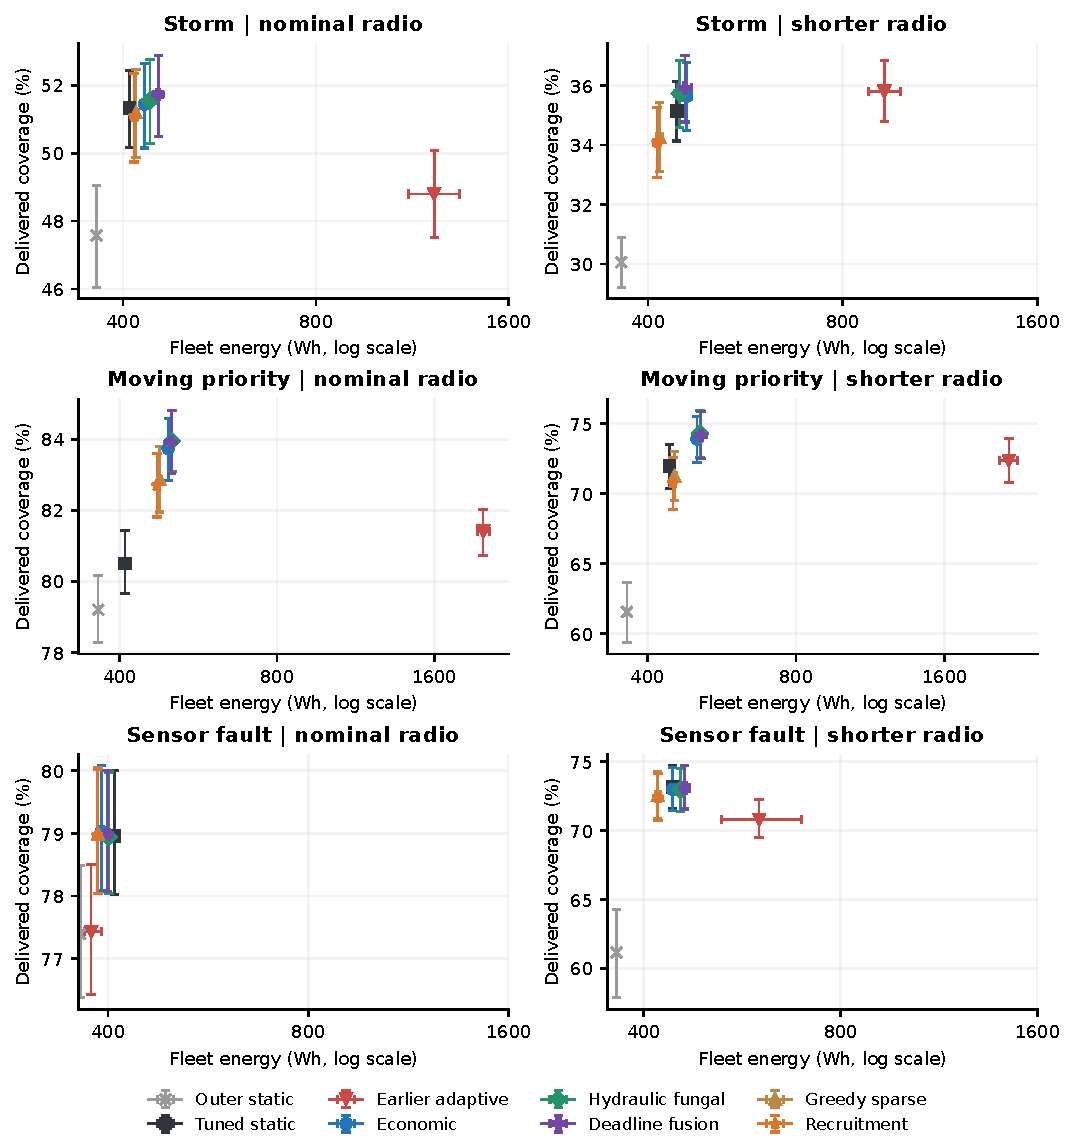
\includegraphics[width=.96\textwidth]{figures/coverage_energy.pdf}
\caption{Coverage--energy outcomes in the six held-out conditions. Each point
summarizes 20 paired missions; bars show 95\% intervals of the mean. Energy uses
a logarithmic axis. Higher coverage and lower energy are preferable.}
\label{fig:pareto}
\end{figure*}

Compared with tuned static, economic control changes coverage by +0.953 percentage points (95\% CI [0.771, 1.129]) and energy by +28.1 Wh ([25.9, 30.3]).

Compared with earlier adaptive, economic control changes coverage by +1.687 percentage points (95\% CI [1.482, 1.901]) and energy by -758.0 Wh ([-796.4, -718.8]).

\begin{figure*}[tbp]
\centering
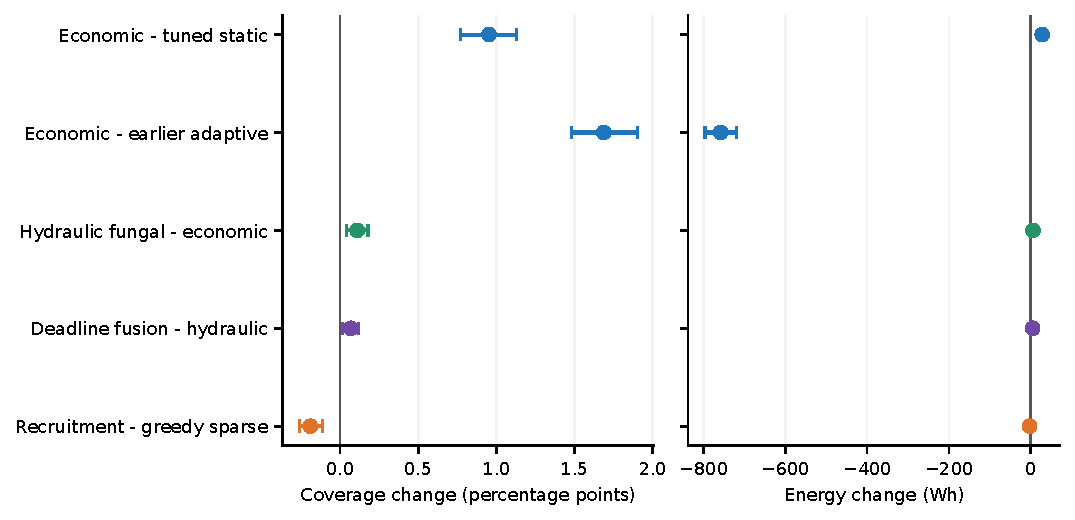
\includegraphics[width=.96\textwidth]{figures/paired_effects.pdf}
\caption{Paired pooled changes. Positive coverage differences are beneficial;
positive energy differences represent extra cost. Intervals resample whole seed
blocks. Biological comparisons are exploratory.}
\label{fig:paired}
\end{figure*}
\subsection{Biological comparisons}

Hydraulic fungal minus economic yields +0.109 coverage points ([0.039, 0.178]; $p_{\mathrm{Holm}}=0.017$) and +5.6 Wh ([3.1, 8.3]).

Deadline fusion minus hydraulic fungal yields +0.068 coverage points ([0.015, 0.120]; $p_{\mathrm{Holm}}=0.025$) and +4.7 Wh ([1.4, 8.1]).

Recruitment minus greedy sparse yields -0.191 coverage points ([-0.263, -0.114]; $p_{\mathrm{Holm}}<0.001$) and -2.7 Wh ([-4.1, -1.3]).

These comparisons concern the complete proposal mechanisms under a common
acceptance objective. A pooled interval does not imply that every scenario
benefits, and equal energy prices do not impose exactly equal realized energy.
The price-sensitivity results provide additional trade-off context.
The effects are heterogeneous. Economic control versus tuned static gains
3.23 coverage points in nominal-radio moving priority and 1.94 points with
shorter radio, but changes coverage by -0.15 points in the shorter-radio
sensor-fault case. Deadline fusion versus hydraulic fusion gains 0.17 and
0.19 points in the two storm cells, while changing coverage by -0.03 and
-0.14 points in the two moving-priority cells. These descriptive cell patterns
suggest conditions for future hypotheses; they are not independently confirmed
subgroup discoveries or a reason to discard unfavorable cells.
\begin{figure*}[tbp]
\centering
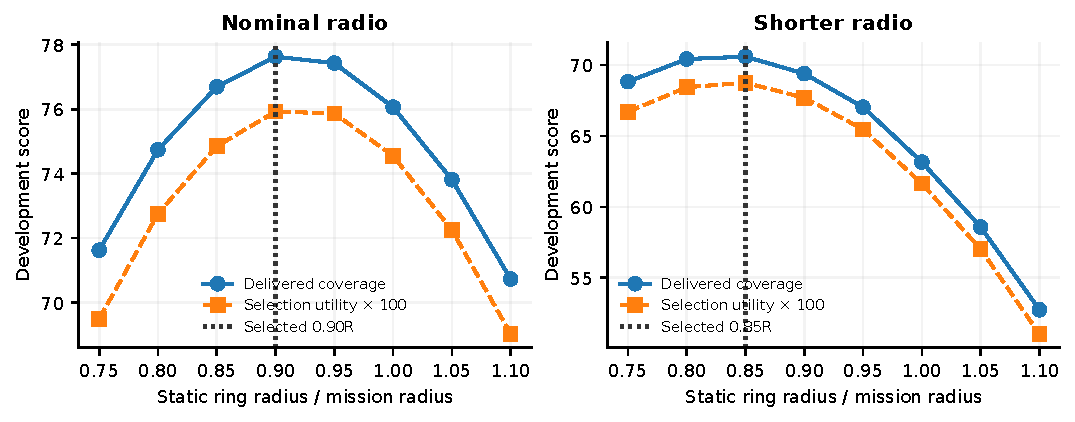
\includegraphics[width=.94\textwidth]{figures/static_selection.pdf}
\caption{Static-design development data, excluded from held-out estimates.
The selected radius differs by radio profile. Coverage and the penalized
selection utility are plotted on a common score scale.}
\label{fig:static}
\end{figure*}
\subsection{Physical trajectories and secondary outcomes}

The main runs recorded 0 collision steps below the simulator's 30 m threshold; the minimum observed pair separation was 690.4 m. This is a measured outcome in these runs, not a formal safety guarantee. Receiver AoI and command staleness are included in Table~\ref{tab:main}; per-scenario secondary outcomes and reference-traffic metrics are retained in the raw data.

\begin{figure*}[tbp]
\centering
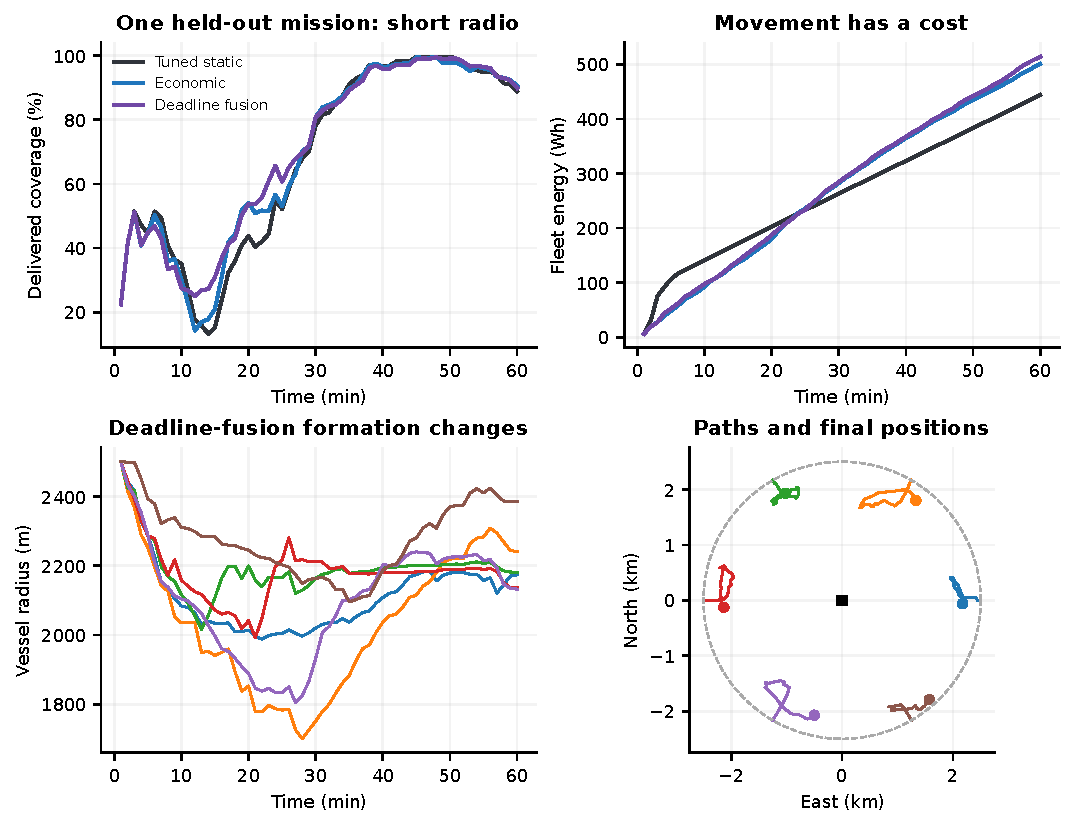
\includegraphics[width=.94\textwidth]{figures/representative_mission.pdf}
\caption{Illustrative held-out seed 7000, moving priority, shorter radio.
The coverage display uses a trailing five-sample average of one-minute trace
samples. Vessel colors agree between the two lower panels; dots mark final
positions. This is one trajectory, not the evidence used to select a winning
policy or a substitute for the paired statistical comparisons.}
\label{fig:trajectory}
\end{figure*}
\subsection{Mechanism, price and model checks}
The frozen diagnostic suite adds 508 missions. These are exploratory checks;
their intervals are pointwise and are not adjusted across all diagnostic tests.
The mechanism checks pair ten seed blocks across storm and moving-priority
conditions with the shorter radio. Figure~\ref{fig:ablation} reports both
coverage and realized energy.
Energy penalty: mechanism present minus removed changes coverage by -0.477 [-0.692, -0.283] points and energy by -49.5 [-59.2, -39.6] Wh.

Hydraulic fusion family: mechanism present minus removed changes coverage by +1.045 [0.817, 1.309] points and energy by -1.0 [-9.0, 7.2] Wh.

Social recruitment: mechanism present minus removed changes coverage by -0.059 [-0.188, 0.086] points and energy by -1.9 [-5.0, 1.2] Wh.

The no-fusion variant replaces mixed directions with branching-only step
lengths; this changes the proposal family as well as removing the hydraulic
term. It is not a perfectly isolated biochemical-mechanism intervention.
Price checks use the same ten seed blocks at three common energy prices.
These curves expose cost--coverage trade-offs, but do not constitute an
exactly energy-matched or globally optimized Pareto frontier.
\begin{figure*}[tbp]
\centering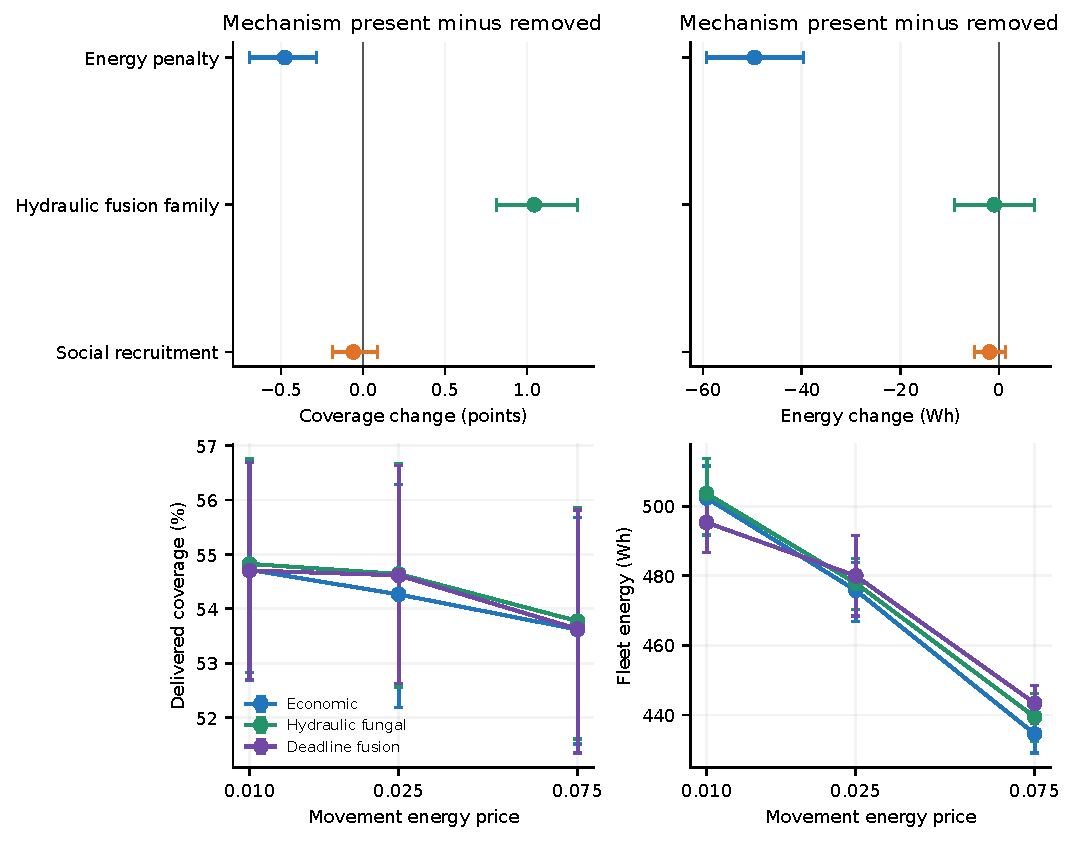
\includegraphics[width=.96\textwidth]{figures/ablation_price.pdf}
\caption{Exploratory mechanism and movement-price checks. Differences use
paired seed blocks; all bars are 95\% bootstrap intervals. Each price point
averages the same ten seeds across two scenarios.}
\label{fig:ablation}
\end{figure*}
\begin{table*}[tbp]
\centering\small\setlength{\tabcolsep}{4pt}
\caption{Diagnostic contrasts with 95\% paired intervals. E: economic; S: tuned
static; H: hydraulic fusion; D: deadline fusion. $n$ counts seed blocks.
Positive energy changes are costs. These are exploratory, pointwise intervals.}
\label{tab:sensitivity}
\begin{tabular}{@{}llrrr@{}}\toprule
Condition & Contrast & $n$ & \shortstack{Coverage change\\(points)} & \shortstack{Energy change\\(Wh)}\\\midrule
\inputtablerows{generated/supplement_table.tex}
\bottomrule\end{tabular}
\end{table*}
Table~\ref{tab:sensitivity} reports altered sensing/correlation, a slower
moving priority, 128-path planning, and calm/blackout controls. The altered-model
case jointly changes the actual detector to a probit curve and increases wave
memory/correlation; it cannot isolate those individual causes. Slower priority
travels at approximately 1.09 m/s, below the 3 m/s vessel limit. The 128-path
check uses only four independent seed blocks and compares policies within that
setting; it is not a paired numerical-convergence test against the 32-path main
study. Negative controls pool the two hardware profiles by seed. A complete
radio blackout prevents delivery irrespective of any formation policy.
The small default biological advantages are not robust across these checks.
Under changed sensing/correlation, both biological coverage intervals include
zero. With slower priority, deadline fusion loses 0.665 coverage points against
hydraulic fusion (interval [-0.934, -0.398]). In the four-seed 128-path check,
hydraulic fusion also underperforms economic control; this small experiment
does not identify numerical integration as the sole cause. Economic control
still improves coverage relative to tuned static in the changed-model and
slower-priority checks, while spending additional energy. These outcomes favor
economic control as the practical baseline and limit claims about biological
performance benefits.

\subsection{Learning pipeline and negative learning result}
A dependency-free linear-softmax REINFORCE policy chooses among nine combinations
of movement step and energy price around the economic controller. Four received
observation frames provide 332 input features for six vessels. The policy sees
cached states, belief summaries and ages, not private true sensor health.
Training uses domain-randomized 40-minute missions. One training seed was run for
50 episodes, evaluated, then resumed for five additional episodes to check
checkpoint continuity. The 50-episode checkpoint is retained separately; the
55-episode checkpoint is not the policy evaluated here.
The 50-episode policy was tested on 18 missions, three scenarios and six paired seed blocks, against constant action 4, which reproduces the neutral economic controller. Coverage changed by -0.805 points (95\% interval [-1.154, -0.397]) and energy by -54.0 Wh ([-80.8, -23.5]). The evaluation utility $\bar C-0.025E/(600\,\mathrm{Wh})$ changed by -0.00581 ([-0.00840, -0.00287]). There is no evidence here that learning improves the mission objective. The energy saving comes with a coverage loss. These small-sample intervals and one training seed do not characterize robust learning performance.
\begin{figure*}[tbp]
\centering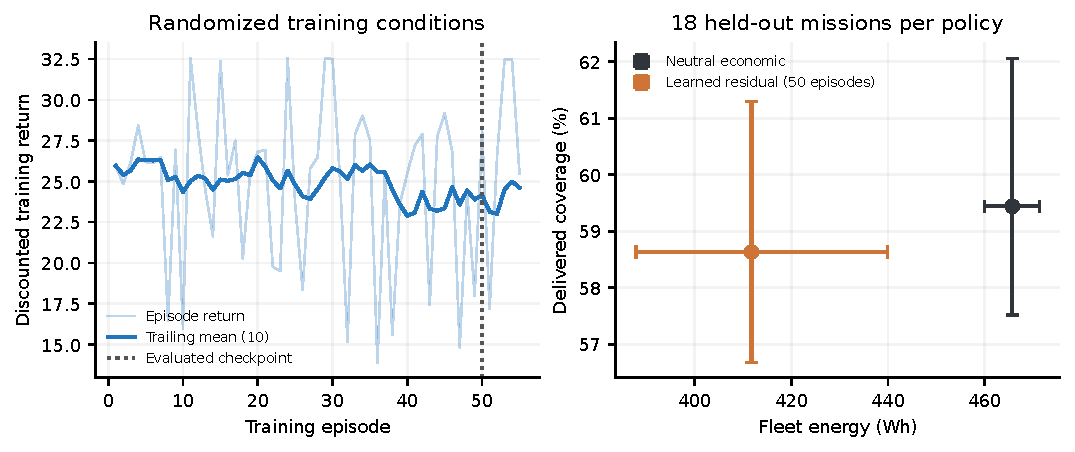
\includegraphics[width=.96\textwidth]{figures/learning.pdf}
\caption{Exploratory learning study. Left: randomized training returns, including
five resume-test episodes after the evaluated checkpoint. A training curve is
not evidence of improved held-out performance. Right: evaluation of the saved
50-episode policy against its neutral economic action; intervals resample six
seed blocks.}
\label{fig:learning}
\end{figure*}
The optional Gymnasium/Stable-Baselines3 PPO environment also passed the
environment checker. PPO was trained for 512 steps, saved, resumed for 128 more,
and loaded for two complete evaluation missions. This 640-step run verifies
the software path only; it is not a substantive PPO efficacy experiment.
The first 512 steps took 129.0 s on the provided CPU environment under concurrent
load (3.97 steps/s). Native training took 505.3 s for the first 50 episodes.
Local hardware should be timed before budgeting longer training.


\FloatBarrier
\section{Further biological mechanisms: a separate experiment}
\label{sec:v4}
The preceding study found small default biological effects that were not robust
across diagnostics. We therefore examined mechanisms that change decision timing
and commitment, retaining the physical simulator and the economic evaluator.
This second experiment uses new world seeds and a shorter, explicitly separate
benchmark. Its absolute coverage values must not be pooled with the earlier
one-hour benchmark.

\subsection{Literature assessment and scope of transfer}
Amichay et al.\ experimentally identified out-of-phase burst timing in juvenile
zebrafish and tested reciprocal temporal coupling in virtual reality. Within a
responsive interval, their phase response is approximated by $T=2\tau$, where
$\tau$ is the lag between a focal burst and its partner's burst~\cite{amichay2024}.
We transfer this timing relation to eligibility for changing a vessel's goal.
The seconds-to-minutes rescaling and pairing of vessel identifiers are engineering
choices, not fitted biological parameters. No hydrodynamic swimming-efficiency
benefit is assumed.

March-Pons et al.\ model threshold-dependent cross-inhibition in honeybee-inspired
decisions~\cite{marchpons2025}. Stronger consensus can trade against choosing the
better option, making benefit in a changing monitoring mission uncertain.
Our adaptation keeps persistent support for ten movement-proposal families.
These are virtual populations inside the coordinator, not ten boats or a
simulation of messages exchanged by biological scouts.

The novelty search also identified cross-inhibition in robot swarms under
biased information~\cite{zakir2026} and a revised 2026 preprint using multi-agent
reinforcement learning to study electric-fish sensing and communication
\cite{singh2026}. These are explicit adjacent precedents. Electrical signal
borrowing is modality-specific: our radar/camera abstraction contains no
corresponding emitter--receiver interaction. We did not insert a free sensor-range
multiplier or claim to have tested that phenomenon. Finding no exact match in this
bounded search would not establish priority over all USV or drone literature.

\subsection{Reciprocal handover eligibility}
Vessels are paired as $(0,1),(2,3),\ldots$ before the mission. A pair becomes
eligible for a fresh excursion only when both cached positions are within
$35$ m of their previously issued goals. At most one member of an eligible pair
can receive a changed goal. The \emph{periodic} comparator alternates eligible
identities each 60-s decision; the \emph{greedy} comparator chooses the member
with the larger coverage-gradient norm. Both share the same settling gate.

For the reciprocal rule, let $b_i$ denote the last accepted goal-change time,
and $d_i$ the next eligible time. Among due members of a settled pair, the oldest
due time wins. When a goal change for $i$ is accepted at time $t$,
\begin{align}
 b_i &\leftarrow t, &d_i&\leftarrow t+120\ \mathrm{s},\\
 \tau_{ji}&=t-b_j, &d_j&\leftarrow b_j+2\tau_{ji}
 \quad\text{if }60\leq\tau_{ji}\leq240\ \mathrm{s}.
\end{align}
Outside this interval, $d_j$ is unchanged. Initially the even/odd members have
$(b_i,d_i)=(-120,0)$ and $(-60,60)$ s, respectively. The relation reproduces
alternating eligible times in an undisturbed two-agent example; it is not a
stability result under delays. Events here are accepted coordinator decisions,
not confirmed physical motion. Cached poses, delayed commands and independent
onboard avoidance preclude a hard guarantee that only one vessel physically
moves in each pair. The simulator does not add a new acknowledgement channel.

All three handover policies use the same ten proposal slots, gradient evaluations,
energy price and acceptance threshold. Ineligible vessels retain their old goals
in every slot, including the stopping proposal. Comparison against unrestricted
economic control measures the whole restriction; reciprocal versus periodic or
greedy handover isolates the timing rule more closely.

\subsection{Nonlinear commitment to movement proposals}
For proposal $a\in\{0,\ldots,9\}$, let $J_a$ be the economic score and
$f_a\geq0$ its virtual committed fraction. A bounded quality input and its
normalized discovery preference are
\begin{align}
 z_a&=\operatorname{clip}((J_a-\max_bJ_b)/0.01,-30,0),\\
 \pi_a&=\frac{e^{z_a}}{\sum_b e^{z_b}},\qquad r_a=\frac{1}{1+4\pi_a},\\
 f_0^{\rm free}&=1-\sum_a f_a.
\end{align}
The subscript zero on $f_0^{\rm free}$ denotes the uncommitted population,
distinct from the committed fraction for proposal index zero. We integrate
\begin{equation}
 \dot f_a=f_0^{\rm free}\bigl[0.5\pi_a+0.5f_a\bigr]
 -r_af_a-f_a\sum_{b\ne a}\sigma(f_b).
\end{equation}
The linear comparator uses $\sigma(x)=x$; the nonlinear rule uses the
linearly bounded sigmoid $\sigma(x)=x/[1+e^{-10(x-0.3)}]$.
The latter response comes from Ref.~\cite{marchpons2025}; the quality mapping,
ten changing proposal families and time scale are our engineering adaptation.
Support starts at zero and persists across decisions. Each decision integrates
two dimensionless time units in 100 explicit Euler steps. Because inflows are
nonnegative on a zero component and total committed outflow returns to the
uncommitted compartment, the continuous dynamics preserve the probability
simplex. The implementation verifies simplex membership without clipping, and
a half-step check tests numerical sensitivity.

The largest committed fraction proposes the action, which is executed only if
its current modeled gain exceeds the same economic improvement threshold.
Persistence attaches to a proposal's \emph{type}, not a fixed geographic location;
changes in proposal geometry are a limitation of this memory. Unchanged sensing,
network and plant models prevent a biology-specific physical advantage by
construction. No distributed consensus or closed-loop coverage theorem is claimed.

\subsection{Frozen evaluation and computational cost}
The new nominal and short-radio profiles each use six vessels, 2400-s missions,
32 angular quadrature points on each of three annuli, and 20 secondary reference
events. The moving priority completes $2/3$ of a revolution per mission, preserving
the earlier angular speed rather than accelerating the front when shortening
the episode. Four scenarios are storm, sensor fault, moving priority and
intermittent conditions. Twelve common world-seed blocks per profile yield
576 main missions across six policies. A 12-mission integration pilot precedes
the freeze and does not select parameters.

Additional diagnostics use a probit physical detector, longer correlated
disturbances and short radio (96 missions, four seeds), and 128 planner paths
(48 missions, four seeds and two scenarios). These remain small diagnostics.
The three declared biological coverage contrasts are reciprocal minus periodic,
reciprocal minus greedy, and nonlinear minus linear inhibition. Bootstrap
intervals resample whole world-seed blocks after averaging the eight main cells;
three pooled coverage tests receive Holm correction. Energy, lower-tail coverage,
AoI, connected-graph frequency and computation are reported separately.

Each unrestricted decision uses $4N$ finite-difference field evaluations and
up to $3K$ trajectory-field evaluations for $K=10$ proposals, plus inexpensive
motion and energy forecasts. Each field evaluation samples $S$ paths over $L$
deadline rounds and $Q$ monitoring locations. Its principal scaling is
$O(SL(N^2+NQ)+N^3)$, including correlated visibility and temporal reachability;
this is not linear scaling in swarm size. The commitment update adds
$O(RK)$ work for $R=100$ internal steps. Equal proposal counts help attribution;
the settling restrictions can nevertheless generate duplicate proposals.
Wall times are measured on a shared CPU host, not as isolated hardware benchmarks.

\subsection{Results of the new mechanism tests}
The second study adds 732 model-based missions, including the pilot and declared diagnostics. Reciprocal versus periodic handover changes coverage by -0.21 [-0.35, -0.09] percentage points and total energy by -5.55 Wh. Relative to greedy handover the coverage contrast is -0.45 [-0.63, -0.28] points. Nonlinear versus linear inhibition changes coverage by +0.01 [-0.04, +0.06] points and energy by -1.48 Wh. Brackets are paired 95\% bootstrap intervals, not predictive bounds for a new vessel platform.
\begin{table}[t]\centering\small
\caption{New main-study means. Each policy has 96 missions across two radio profiles and four scenarios.}
\begin{tabular}{lrrr}\toprule Policy & $\bar C$ & $E$ [Wh] & AoI [s]\\\midrule
Economic & 0.6957 & 300.9 & 49.3 \\
Periodic handover & 0.6843 & 280.1 & 51.0 \\
Greedy handover & 0.6867 & 282.9 & 50.6 \\
Reciprocal handover & 0.6822 & 274.5 & 51.2 \\
Linear inhibition & 0.6962 & 301.0 & 49.4 \\
Nonlinear inhibition & 0.6963 & 299.5 & 49.3 \\
\bottomrule\end{tabular}\label{tab:v4means}\end{table}
\begin{figure*}[tbp]\centering
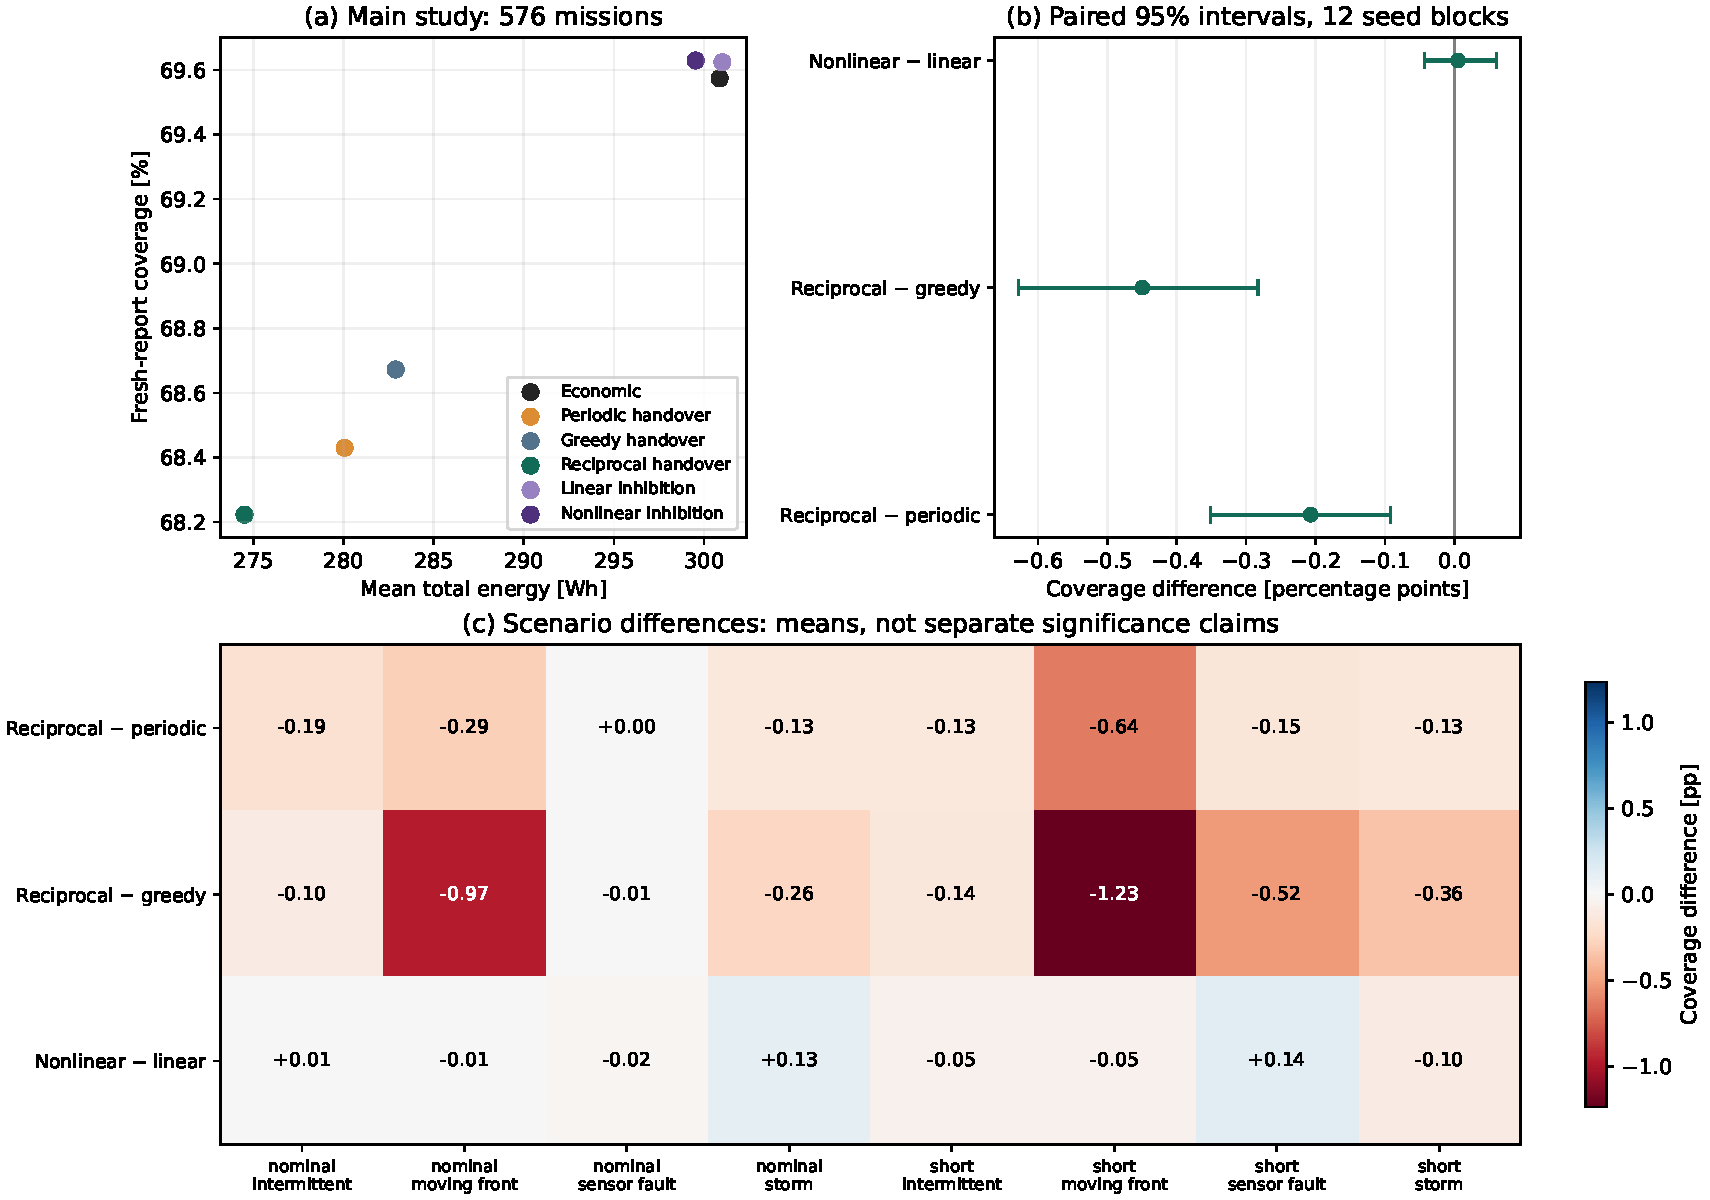
\includegraphics[width=.97\textwidth]{figures/bio_mechanisms.pdf}
\caption{Additional biological mechanisms with matched restrictions. Main-study coverage--energy means, paired coverage contrasts, and scenario-specific differences. A reduced movement budget can save energy while losing timely monitoring.}
\label{fig:v4bio}\end{figure*}
\begin{table*}[tbp]\centering\small
\caption{Prespecified new biological contrasts and small diagnostics. Coverage differences are in percentage points, with paired 95\% intervals. Main $p_H$ values apply Holm adjustment to three coverage tests; diagnostics are descriptive.}
\begin{tabular}{llrrr}\toprule Setting & Contrast & $\Delta C$ [95\% interval] & $\Delta E$ [Wh] & $p_H$\\\midrule
Main, 12 blocks & Reciprocal -- periodic & -0.21 [-0.35, -0.09] & -5.55 & 0.008 \\
Main, 12 blocks & Reciprocal -- greedy & -0.45 [-0.63, -0.28] & -8.38 & 0.002 \\
Main, 12 blocks & Nonlinear -- linear & +0.01 [-0.04, +0.06] & -1.48 & 0.850 \\
Shifted, 4 blocks & Reciprocal -- periodic & -0.28 [-0.59, +0.04] & -3.28 & -- \\
Shifted, 4 blocks & Reciprocal -- greedy & -0.36 [-0.67, -0.16] & -5.35 & -- \\
Shifted, 4 blocks & Nonlinear -- linear & -0.07 [-0.14, -0.00] & +0.46 & -- \\
128 paths, 4 blocks & Reciprocal -- periodic & +0.03 [-0.41, +0.47] & -6.16 & -- \\
128 paths, 4 blocks & Reciprocal -- greedy & -0.58 [-0.74, -0.42] & -6.32 & -- \\
128 paths, 4 blocks & Nonlinear -- linear & -0.01 [-0.21, +0.18] & +0.33 & -- \\
\bottomrule\end{tabular}\label{tab:v4contrasts}\end{table*}
These adaptations should be judged against their matched controls and against unrestricted economic control. Reciprocal handover versus economic control changes coverage by -1.35 [-1.60, -1.13] points; nonlinear inhibition versus economic control changes it by +0.06 [-0.03, +0.16] points. A small main-study contrast alone does not establish a generally useful biological advantage. The changed observation law and integration resolution are particularly relevant because all policies still optimize a sampled, imperfect prospective score.


\subsection{Why a biological transfer may not help here}
The simulator allows sensing throughout motion; it has no fitted motion-induced
sensor-blind interval. Moreover, the coordinator already computes all ten
prospective scores. Temporal alternation therefore incurs a mobility restriction
without necessarily gaining the sensory-processing advantage that motivates it
in fish. Virtual consensus does not acquire independent local evidence that
the centralized argmax comparator lacks. These are properties of the engineering
mapping, not evidence against the biological findings.

A post-hoc inspection of the eight presaved nonlinear-inhibition main missions (world seed 17000, two profiles and four scenarios) found that only 1.29\% of 310 nonstale decisions had any proposal fraction above the 0.3 sigmoid midpoint; mean maximum support was 0.091. The threshold was borrowed from a primarily binary-choice biological model, whereas these ten often similar movement proposals fragment support. This is a descriptive diagnosis, not a causal ablation: lower thresholds or grouping proposals into meaningful alternatives require a separate development and test experiment.


This suggests testing the placement of a mechanism before expanding its
complexity: a distributed information bottleneck, calibrated sensing interruption
or explicit decision-consensus requirement would have to be represented and
costed. Adding such a feature solely to favor the biological method would be
invalid. A new application model needs independent justification and new matched
controls. The current negative results should remain part of that record.

\subsection{Reinforcement learning: what is learned and how it is compared}
The executable learner selects one of nine pairs of movement step
$\{60,120,180\}$ m and economic price $\{0.0125,0.025,0.05\}$ at 60-s intervals.
It does not learn navigation, collision avoidance, task allocation or sensing
physics. Action 4 exactly recovers the standard economic controller.
Four cached observation frames feed the unchanged PPO adapter. Domain
randomization varies radio/sensor nominal ranges and mission scenarios; no true
hidden sensor health is supplied to the policy.

Three independent training seeds receive 2048 steps each, still a short pilot.
For comparison, all nine constant settings are evaluated on three separate
development world seeds in four scenarios, and the setting with the highest
mean undiscounted step reward is fixed. Every trained seed, that selected setting
and neutral action 4 are then compared on eight new world seeds. We report
discounted return, mean step reward, post-warmup coverage and actual energy
separately: training uses discounted rewards whereas the development selection
uses their undiscounted mean. Longer training is not assumed to improve test
performance~\cite{sb3tips}.

The development set selected constant action 3: a 120-m proposal step and price 0.0125. Against that setting, the mean of the three short PPO policies changes mean interval reward by -0.00607 [-0.00743, -0.00449], post-warmup coverage by -0.87 [-1.03, -0.69] percentage points and energy by -44.84 [-48.44, -41.46] Wh. These intervals resample eight mission-seed blocks while keeping the three learned policies fixed; they do not quantify performance across the population of possible training runs.
\begin{table}[t]\centering\small
\caption{Held-out short-PPO evaluation: 32 missions per policy, after 2048 steps per training seed.}
\begin{tabular}{lrrr}\toprule Policy & Mean reward & $\bar C$ & $E$ [Wh]\\\midrule
constant 3 & 0.6259 & 0.6348 & 329.2 \\
constant 4 & 0.6255 & 0.6331 & 310.4 \\
ppo seed0 & 0.6168 & 0.6217 & 261.9 \\
ppo seed1 & 0.6259 & 0.6348 & 329.2 \\
ppo seed2 & 0.6168 & 0.6217 & 261.9 \\
\bottomrule\end{tabular}\label{tab:v4rl}\end{table}
\begin{figure*}[tbp]\centering
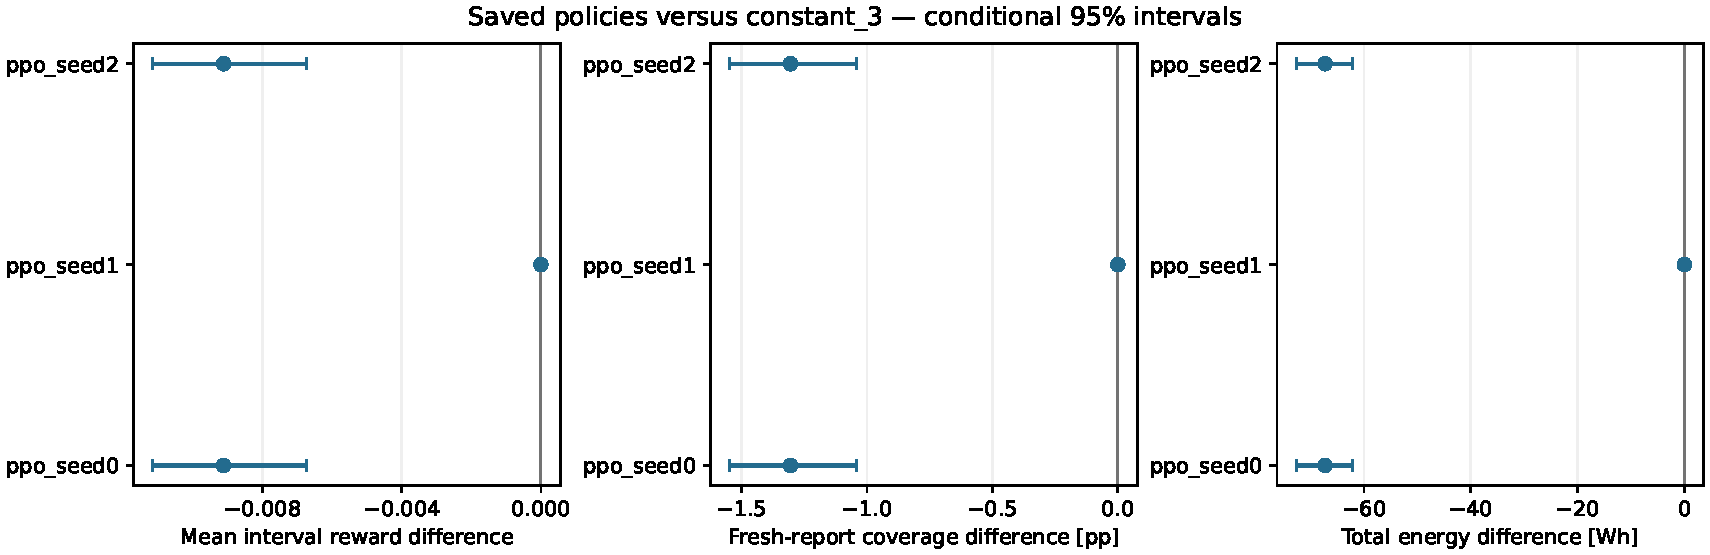
\includegraphics[width=.98\textwidth]{figures/ppo_v4.pdf}
\caption{Each short PPO training seed compared with the development-selected constant setting on the same held-out world seeds. Intervals condition on the trained policies. Favorable energy differences are negative; favorable reward and coverage differences are positive.}
\label{fig:v4ppo}\end{figure*}
The three training runs completed at 2.74--3.70 steps/s on a shared CPU. A separate 256-step, two-chunk run exercised the progress wrapper and optimizer continuation. Neither that software check nor a 2048-step pilot establishes convergence. The useful deliverable is a reproducible way to test learning against strong fixed settings, with no guarantee that extra training improves coverage or reward.
Action logs show that ppo seed0 used action 1 at every evaluated decision; ppo seed1 used action 3 at every evaluated decision; ppo seed2 used action 1 at every evaluated decision. This observed constant behavior provides no evidence of learned state-dependent adaptation, even when its score matches a strong fixed setting.


The Windows handoff adds chunked checkpoints, explicit progress, a machine-specific
runtime estimate and development/test scripts. Resuming restores PPO parameters,
optimizer and step count but restarts environment trajectories. The current continuation runner assigns a distinct, recorded environment stream to each chunk, derived from the training seed and completed step count. This prevents deliberate replay of the same initial seed sequence. Chunk boundaries
therefore change the training experiment; chunked and uninterrupted runs are not
claimed identical. The reported 2048-step pilots use one uninterrupted chunk each.

\section{Interpretation and practical research direction}
\subsection{What constitutes an improvement}
The most consequential engineering change is making each manoeuvre answer to
its expected delivered-information benefit and movement cost. A controller can
improve a spatial sensing score while spending disproportionate time and power
reaching its chosen formation. Small physically attainable proposals provide
a useful alternative. The old and new controllers have different action
families, so their comparison supports the new \emph{control architecture};
it does not establish that a particular biological rule caused the gain.

The tuned static comparator is essential. Choosing a better fixed radius can
recover a substantial amount of performance without continuous adaptation.
An adaptive controller that contracts once and stays there has discovered a
static design, not demonstrated ongoing response intelligence. Reporting
waypoint updates, trajectories and the development-selected static result
helps distinguish those explanations.

Hydraulic fusion expresses a sensible long-term transport preference, but
physical radio reports travel on discrete, time-varying paths. A highly
conducting expected network may still miss a short deadline. Conversely,
a network with mediocre instantaneous connectivity can deliver reports by
waiting for later links. Equation (\ref{eq:influence}) makes that difference
explicit. Its derivation is exact for the stipulated conditional model,
while its sampled estimate, its mapping to vessel movements and its practical
value remain separate questions.

For example, a single report must traverse three consecutive links, each
with independent success probability $q$ per round. Its delivery probability
within $L$ rounds is
$\Prb\{\operatorname{Binomial}(L,q)\geq3\}$.
It is zero for $L<3$, regardless of how hydraulically important those links
appear. This simple counterexample explains why hydraulic importance should
not be substituted for deadline reliability.

\begin{figure}[t]
\centering
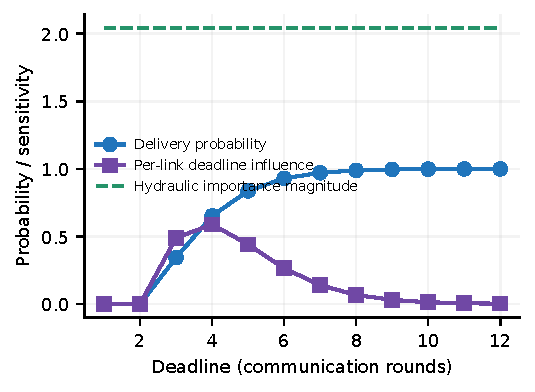
\includegraphics[width=\columnwidth]{figures/deadline_example.pdf}
\caption{An exact three-hop example separates persistent-flow importance from
deadline sensitivity. One report originates before the first round; each round
allows one forwarding hop. Curves are analytical, not additional USV trials.
The electrical analogy assigns importance even when timely delivery is impossible.}
\label{fig:deadline_example}
\end{figure}

\subsection{Limits of the biological interpretation}
The fungal implementation transfers a division of functions: spatial expansion,
transport reinforcement and rejection of redundant expenditure. It does not
simulate fungal tissue, consume construction material, reproduce a travelling
wave, or inherit the biological model's near-Pareto behavior. Ant recruitment
transfers activity-dependent participation; it does not establish that a
liquid-brain mechanism is necessary or best for radio-linked vessels.
Biology is therefore a source of falsifiable proposal mechanisms.

Failure to beat a conventional matched control is scientifically informative.
The coupled activity can preserve a useful role allocation under noisy
observations, but it can also delay a needed change or allocate work according
to obsolete conditions. A global performance gain does not identify the
social term as causal without its ablation. More neuron-like dynamics,
spiking models or evolutionary tuning would introduce additional hypotheses;
none should be added solely to make the method sound more sophisticated.

\subsection{What must be calibrated before deployment}
Three gaps dominate the distance between these results and practical use.
First, sensor curves must come from known objects, ranges and environmental
conditions, with detection and false-alarm definitions fixed in advance.
Availability and range should be estimated jointly; a sequence of distant
misses is often uninformative about which one degraded. An intervention that
improves parameter estimation is worthwhile only if its expected mission value
exceeds its cost. Information gain alone is not that value.

Second, radio tests need packet timestamps, retries, traffic load, antenna
geometry and common-outage measurements. The present ideal cache network has
no finite throughput; 192 virtual monitoring points do not imply a measured
192-object traffic load. A realistic network extension should test
finite-capacity scheduling and distinguish direct base delivery, relay
delivery and command acknowledgement.

Third, a fitted marine dynamics model should predict the energy and timing of
station keeping and formation changes. The present power law,
$60+18|u|^3+8v^2+4r^2$ W, is a declared synthetic model.
Replacing it by vessel-specific hydrodynamics and actuator data could change
the preferred formation policy. A marine-craft model provides an appropriate
structure for that work~\cite{fossen2021}.
Near-field repulsion and sampled separation checks are not COLREGs reasoning,
formal safety filters or evidence of seaworthiness.

\subsection{A bounded route to stronger mathematics}
The original requirement also needs a distinction between continuous graph
connectivity and timely delivery. These experiments improve delivered freshness;
they do not enforce an always-connected graph. Let $\mathcal E_D(g)$ denote the
event that every required vessel has a causal path to the base within $D$.
A future constrained controller could require a calibrated lower bound on
$\Prb\{\mathcal E_D(g)\}$ to exceed $1-\alpha$, or impose an explicit instantaneous connectivity constraint
when that is the actual mission requirement. Such a problem needs feasibility
handling: under a total blackout, a positive reliability requirement is
infeasible. An appropriate fallback would report the outage and preserve local
data, rather than treat the constraint as satisfied. This constraint and its
calibration are proposed future work, not implemented guarantees.

The next mathematical extension should attach a model-error allowance to
the acceptance decision. If, for every compared action,
$|\widehat J(g)-J^\star(g)|\leq\delta$, then accepting only when
$\widehat J(g)-\widehat J(g_0)>2\delta$ ensures a positive difference in
$J^\star$. This follows directly from two applications of the error bound.
The difficult research task is obtaining a valid $\delta$ under delayed
telemetry, health uncertainty and model mismatch. The present implementation
does not possess such a bound.

One practical route is a separately calibrated probability model and an
independent rollout bank for candidate validation. A confidence interval for a
sample average only controls integration error under the assumed model; it
does not cover unmodeled radio interference or sensor clutter.
Distributionally robust planning or calibrated ambiguity sets could address
part of that gap. Such an extension should be compared with a conventional
robust local controller using the same information and uncertainty budget.

To scale the deadline-fusion calculation, cache backward-reachability states
and skip edge-round interventions that cannot alter useful source reachability.
The exact finite-network enumeration test provides a regression oracle for
that optimization. A faster implementation with preserved conditional
expectations would be a concrete addition, even if the biological interpretation
itself does not improve fleet-level outcomes.

\subsection{Learning as a controlled extension}
Learning should address a residual choice that the model-based controller
cannot set well across conditions: step length, energy price, forecast horizon
or a small proposal mixture. Observation history can help infer persistent
degradation from delayed measurements. The released residual adapter exposes
cached per-vessel geometry, belief moments, ages, energy, previous waypoint
errors and global mission context. It adds no hidden-health observation.

A linear history policy is intentionally a transparent baseline. More training
does not guarantee it will outperform the fixed economic rule.
The short PPO study in Section~\ref{sec:v4} adds multiple training seeds and constant-setting controls. A subsequent PPO or recurrent-policy experiment should compare one versus four observations,
domain randomization on/off, multiple training seeds and the best constant
residual action selected on development data. Its evaluation must retain the
movement and communication constraints. Success on a training reward or a
single checkpoint is insufficient evidence of practical learning value.

\subsection{Publication position}
This package is a reproducible simulation manuscript with explicit hypotheses,
negative comparisons and inspectable mathematics. It is ready to be reviewed
and versioned as a research repository. It is not evidence of journal acceptance
or of first use of these ideas in robotics. A journal-strength next version
should make one narrow claim, reproduce closer optimization baselines, and
validate a relevant physical model or hardware-in-the-loop implementation.
For an internship, the strongest immediate product is the measured
coverage--energy decision workflow and the experiments it makes possible.

\section{Conclusion}
Formation adaptation should be evaluated at the receiver, with physical movement
costs and causal report delivery included. This study supplies a common economic
controller, biologically motivated proposal families and a deadline-sensitive
link-importance transfer, evaluated against development-selected static geometry
and conventional controls. The economic controller achieves the clearest
coverage--energy improvement over the earlier adaptive architecture. The small
pooled biological gains are not robust across the diagnostic settings, and the
first evaluated residual learner does not improve the mission objective.
The deadline-influence formulation remains an inspectable research mechanism,
not an established performance breakthrough. The next practical step is calibration and validation of the
sensing, channel and movement models, followed by a fresh held-out comparison.

\section*{Data, software and preparation}
The accompanying repository contains the complete simulation source,
configuration files, raw episode records, analysis scripts, figures, this
\LaTeX{} manuscript, and a staged local run guide. Core physical-simulator and
experimental-controller hashes are recorded separately. External PPO dependencies are optional for ordinary simulation; both the NumPy learning baseline and the additional short PPO runs were executed. Code, literature triage and manuscript preparation used an AI assistant;
the release is intended for independent inspection and human scientific review.
No field experiment, journal acceptance or independently certified novelty is
reported.
\FloatBarrier
\bibliographystyle{unsrt}
\bibliography{references}
\appendix
\begin{table}[tbp]
\centering\scriptsize\setlength{\tabcolsep}{3pt}
\caption{Secondary main-study outcomes, pooled across all six cells. The
coverage percentile is calculated within each mission, then averaged; the three report columns are percentages.
Runtime is mean elapsed time per worker mission under concurrent load;
it is not isolated CPU time or a worst-case control-cycle bound.}
\label{tab:secondary}
\begin{tabular}{@{}lrrrr@{}}\toprule
Policy & P10 $C$ & $C<0.5$ & Early & Runtime (s)\\\midrule
\inputtablerows{generated/secondary_table.tex}
\bottomrule\end{tabular}
\end{table}
\section{Reproduction and parameter details}
The repository root contains \texttt{usv\_sim/} (the unchanged physical
simulator), \texttt{usv\_research/} (preserved controllers and learning), \texttt{usv\_bio/} (additional mechanisms and training drivers), \texttt{configs/}, \texttt{tests/}, \texttt{results/} and
\texttt{paper/}. Full commands appear in the repository's local run guide.
The study-reproduction script reruns the declared held-out suite and retains
existing complete episodes.
Figures and numerical manuscript text are generated by the analysis/figure
scripts, not transcribed from a plot by hand.

Vessel-specific initial radar multipliers are uniform on $[0.82,1.18]$;
availability offsets are Gaussian with standard deviation 0.25.
Camera multipliers are uniform on $[0.9,1.1]$ and the radio episode multiplier
on $[0.92,1.08]$. In the fault case, vessel 0's radar multiplier becomes 0.43
of its original value and its availability offset decreases by 1.15.
For moving priority, the unnormalized angular weight is
\begin{equation}
 \widetilde w(\theta,t)=0.35+
 2.5\exp\{3[\cos(\theta-\Omega t)-1]\},
\end{equation}
where $\Omega=2\pi/T$ by default. All weights are normalized across the
three annuli. A longer mission with the same number of revolutions has a
slower priority front, so duration and front speed must not be conflated.

The actual common radio fade has bad-state persistence
$e^{-\Delta t/25}$ and good-to-bad transition probability
$1-e^{-\Delta t/400}$. The planner uses the corresponding stationary initial
mixture. The simulator starts in the good state and uses a finite spatial
Fourier field for visibility, another reason that its predictor is an
approximation despite shared nominal parameters.

The current is a smooth two-dimensional signal plus a severity-dependent
component. Guidance compensates for the modeled current. Surge speed is capped
at 3 m/s, yaw rate command at 0.25 rad/s, and surge acceleration at
0.25 m/s$^2$. The low-level model has yaw-rate and surge-response time
constants, and stochastic sway. Its onboard repulsion begins within 180 m;
an encounter below 30 m is counted as a collision step. The energy parameter
limits commanded propulsion after depletion, but does not implement a complete
sensor/radio power shutdown. Thus long-horizon battery behavior also requires
further validation.

Thirty-six moving reference craft provide a secondary event metric. Speeds are
uniform on $[4,7]$ m/s. Inward crossing deadlines are constructed independently
of detection and require a report 60 s before crossing radius 1800 m.
Never-reported eligible craft remain failures; a later outbound observation
cannot count as early success. The planner optimizes delivered annular
freshness, not this event-specific measure, so the two outcomes can disagree.

\section{Interpreting file identities and repeat runs}

Table~\ref{tab:secondary} separates tail coverage, event-specific reports and
computation from the primary mean-freshness outcome. Mean deadline-fusion
runtime was approximately 2.73 times that of economic control in the concurrent
main batches. That extra cost matters when assessing its small pooled coverage
gain. The experiment does not establish a hard real-time deadline for every
controller invocation or scaling beyond the tested six vessels.

Each main/sensitivity episode stores its scenario, seed, full configuration,
controller settings, physical-code hash and extension-code hash. Shared
exogenous tape hashes support pairing checks. The released manifest and
verification script check record completeness and source consistency.
An episode-level bootstrap measures stochastic variability inside the stated
model. It cannot turn synthetic assumptions into field evidence.

The native residual learner commits complete episodes with its weights, Adam
state, return baseline, random-generator state and configuration/source
metadata. Exact continuation is checked at a completed-episode boundary.
Optional PPO continuation restores the policy and optimizer but restarts
environment trajectories; it is not advertised as bitwise reproducible
continuation. Training seeds and held-out evaluation seeds are separate.

\end{document}
